\clearpage
\subsection{Task 2.2 -- Sequence diagram}

\subsubsection{Luồng UC-01 từ giỏ đến biên nhận}
Năm lifeline gồm khách hàng, Next.js UI, NestJS API, PostgreSQL và PayOS. Sơ đồ thể hiện kiểm tra giỏ, tạo đơn với phiên JWT, transaction giữ nguyên liệu, hai nhánh thanh toán và kết quả hiển thị. Khi mở checkout, giao diện tải trạng thái và chi tiết đơn song song như trong Activity Diagram. Các khung tham chiếu dẫn đến sơ đồ chi tiết.

\begin{center}
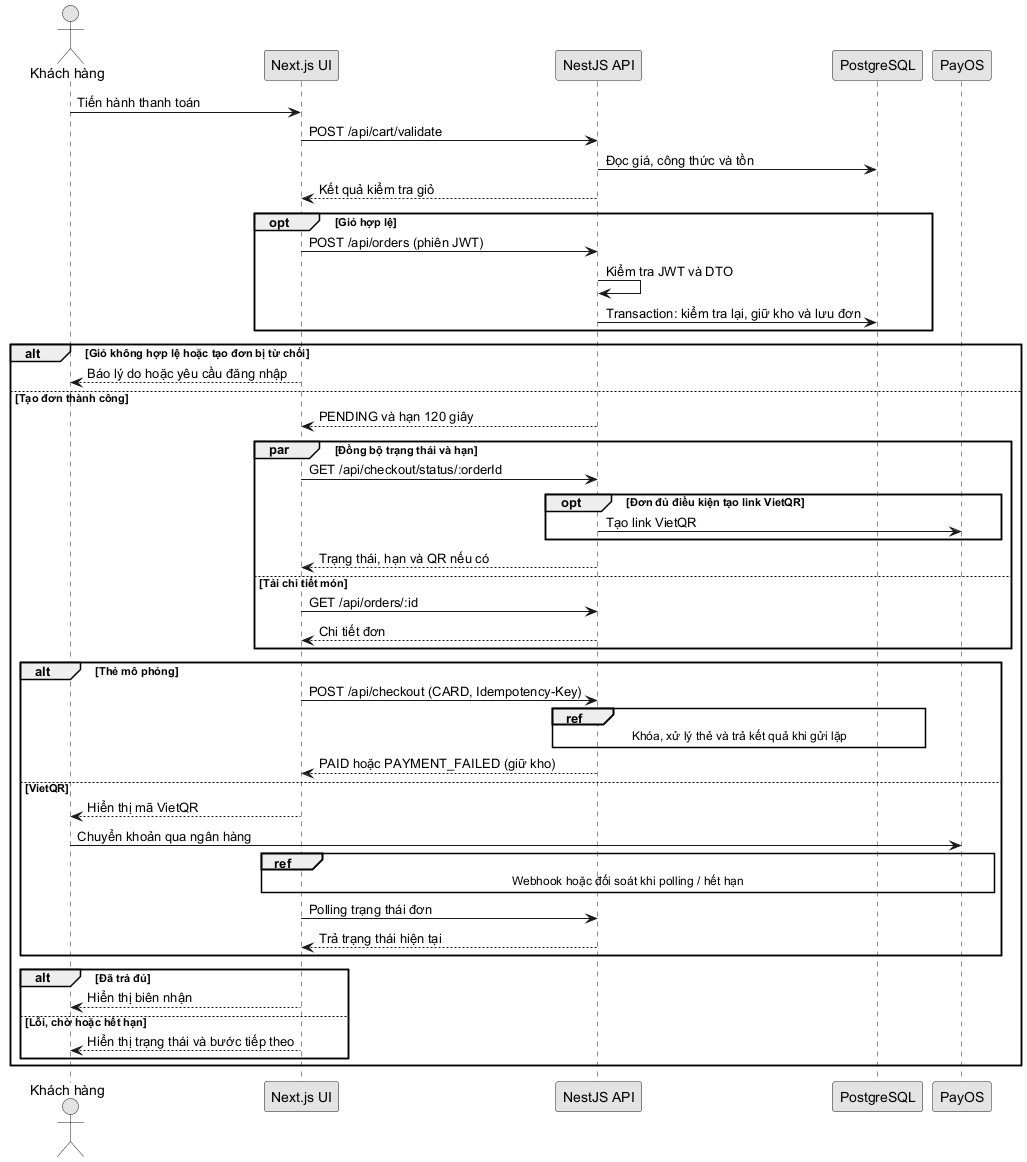
\includegraphics[width=\linewidth,height=0.70\textheight,keepaspectratio]{../../diagrams/sequence-checkout-overview.png}\\[0.5em]
{\small\itshape Hình 2.2a. Trình tự đặt và thanh toán đơn hàng}
\end{center}

\clearpage
\subsubsection{Tạo đơn và tạm giữ nguyên liệu}
Bước kiểm tra giỏ chỉ đọc dữ liệu. API tạo đơn yêu cầu JWT, kiểm tra DTO, tính giá và ưu đãi ở máy chủ, kiểm tra lại giá rồi giữ nguyên liệu bằng cập nhật có điều kiện trong transaction. API trả \texttt{id}, \texttt{total}, trạng thái \texttt{PENDING} và \texttt{reservationExpiresAt}.

\begin{center}
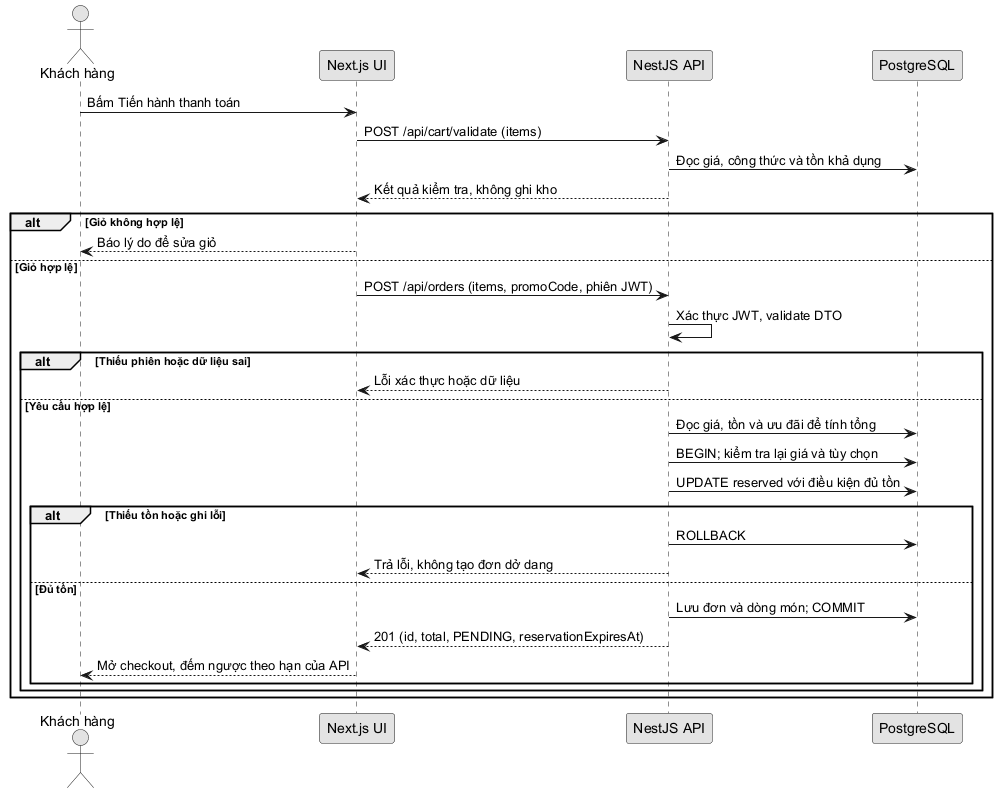
\includegraphics[width=\linewidth,height=0.70\textheight,keepaspectratio]{../../diagrams/sequence-order-reservation.png}\\[0.5em]
{\small\itshape Hình 2.2b. Kiểm tra dữ liệu, khóa nguyên liệu và tạo đơn}
\end{center}

\clearpage
\subsubsection{Chống xử lý lặp khi thanh toán thẻ}
API tra \texttt{Payment.idempotencyKey}. Nếu chưa có kết quả, transaction dùng khóa theo key và khóa dòng đơn, rồi kiểm tra lại để xử lý các yêu cầu đồng thời. Kết quả trả về dựa trên bản ghi \texttt{Payment}. Lượt thử sau thất bại dùng khóa mới nếu đơn còn hạn.

\begin{center}
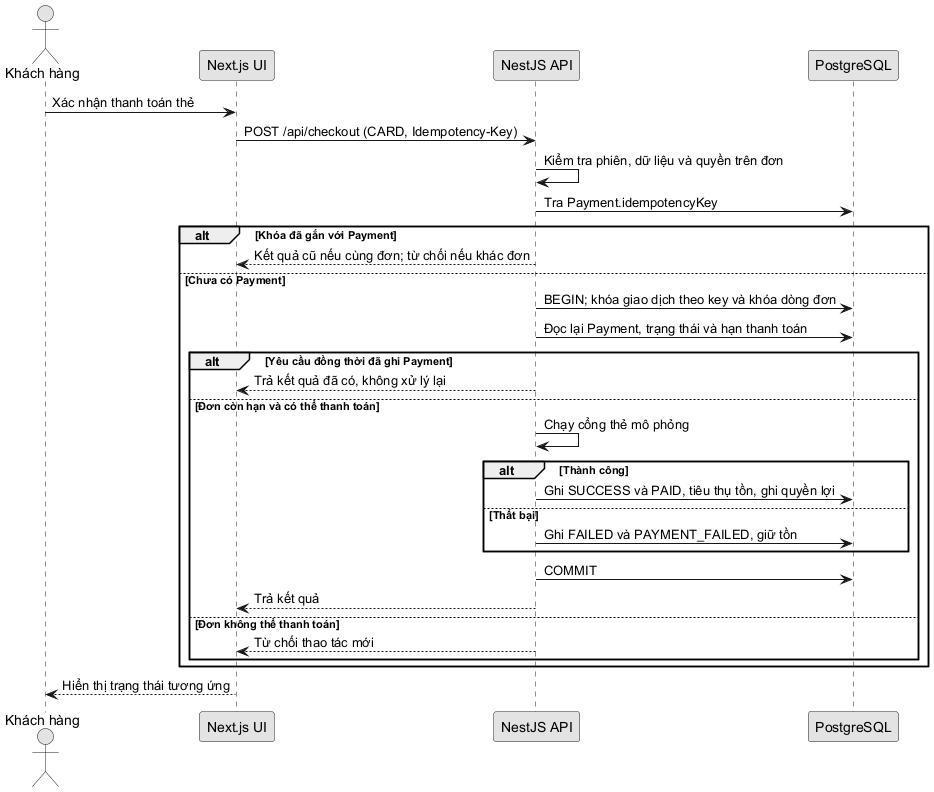
\includegraphics[width=\linewidth,height=0.70\textheight,keepaspectratio]{../../diagrams/sequence-idempotency.png}\\[0.5em]
{\small\itshape Hình 2.2c. Khóa transaction và trả lại kết quả đã ghi}
\end{center}

\clearpage
\subsubsection{Thanh toán VietQR và đối soát PayOS}
PayOS gửi webhook có \texttt{data} và \texttt{signature} trong body. API dùng SDK PayOS kiểm tra chữ ký và đối chiếu giao dịch với đơn. Polling hoặc tác vụ hết hạn cũng có thể đọc trực tiếp trạng thái link. Webhook hợp lệ và polling đồng thời chỉ hoàn tất đơn một lần.

\begin{center}
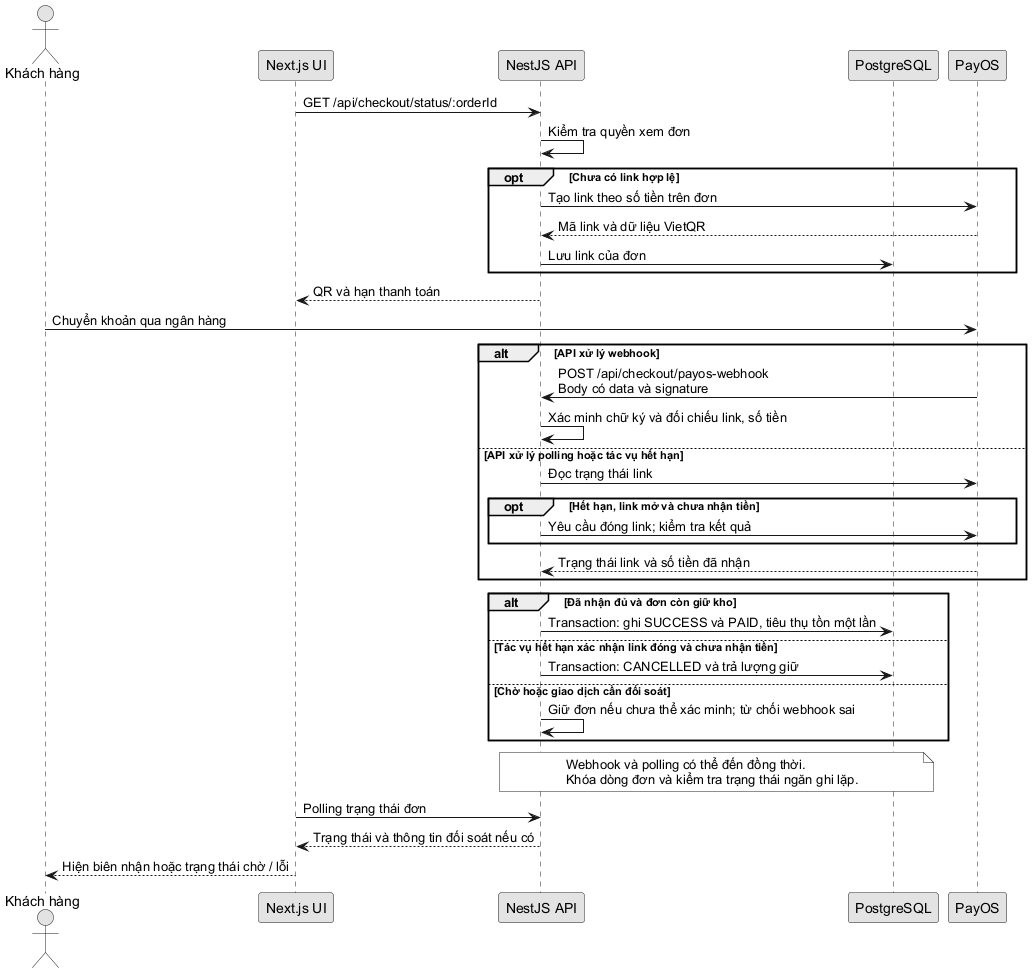
\includegraphics[width=\linewidth,height=0.70\textheight,keepaspectratio]{../../diagrams/sequence-payos-webhook.png}\\[0.5em]
{\small\itshape Hình 2.2d. Xác thực webhook, polling và đối soát khi hết hạn}
\end{center}
